\begin{figure}
\centering
\begin{tikzpicture}
    \draw (0, 0) node[inner sep=0] {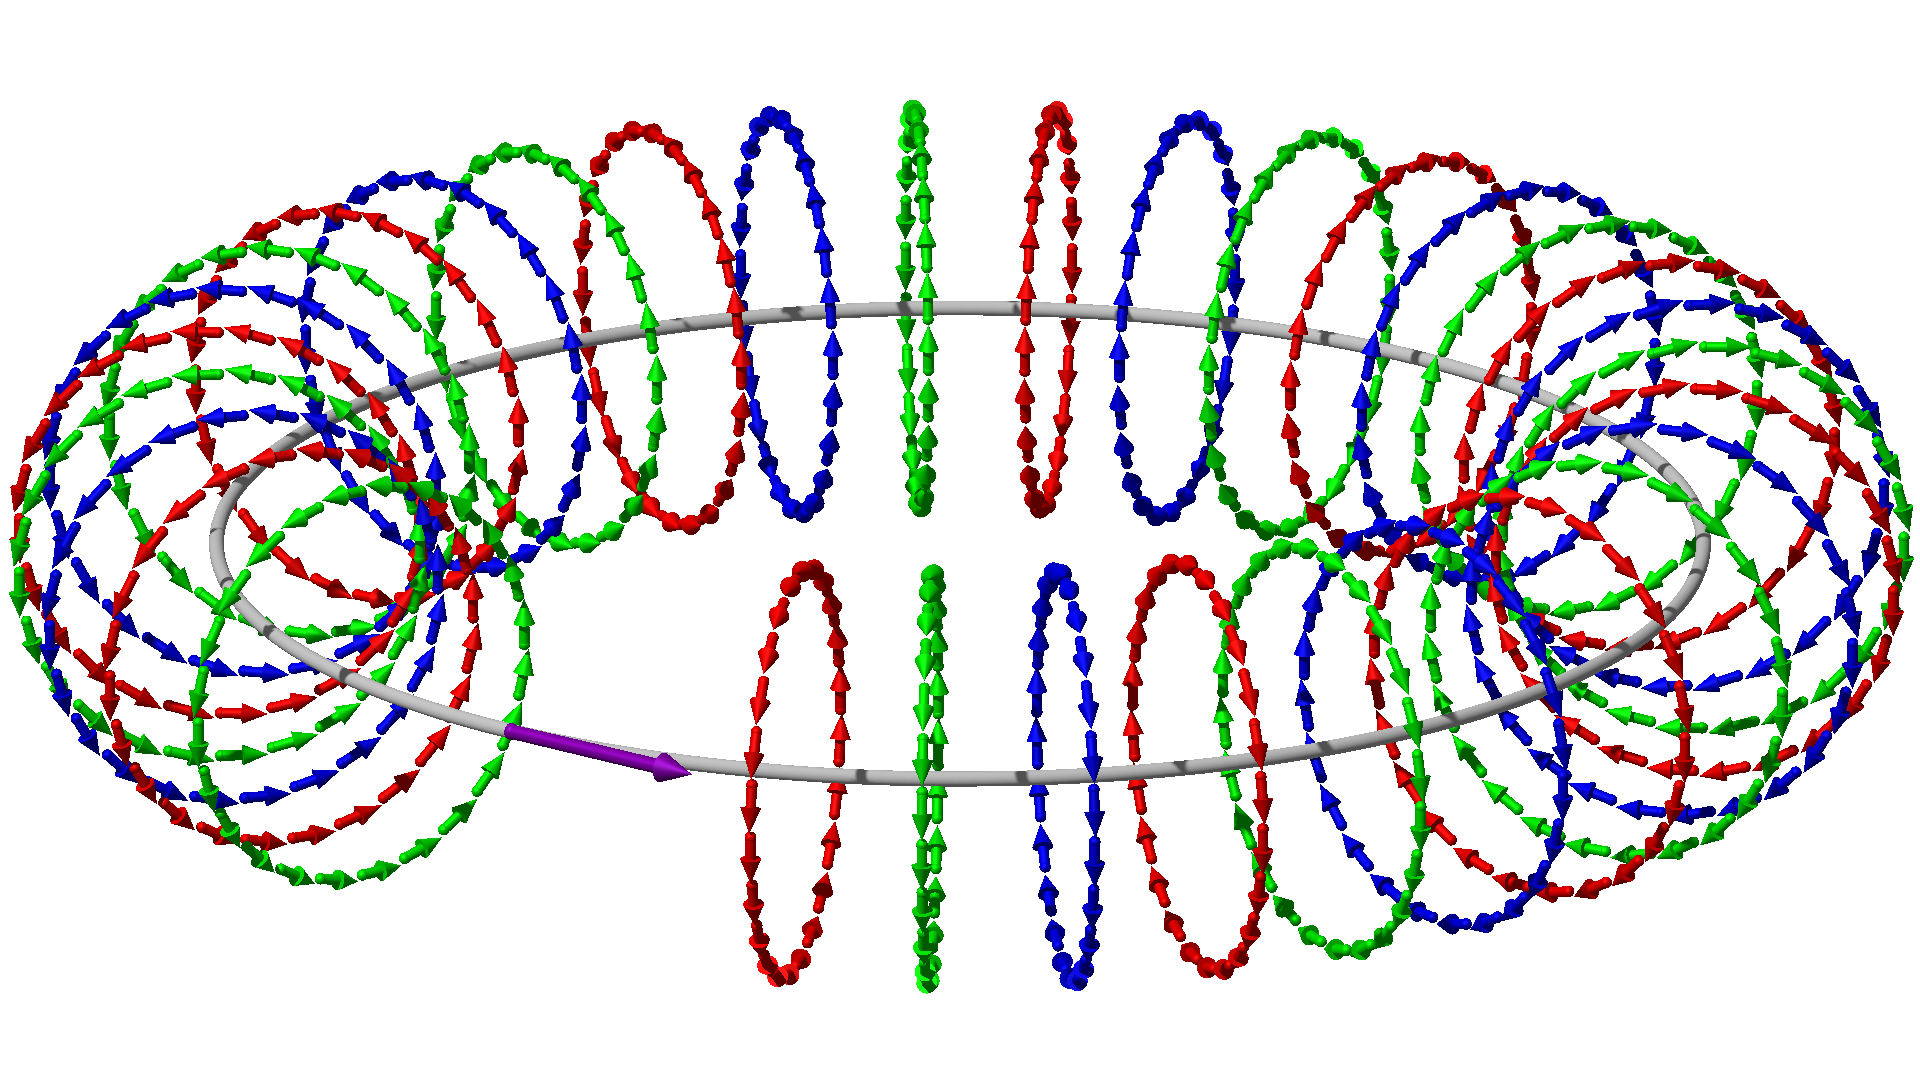
\includegraphics[width=1\textwidth]{papers/wirbelringe/fig/wirbelring_RGB.jpg}};
    \draw (-2.3, -1.05) node {\(\vec{\omega}\)};
\end{tikzpicture}
\caption{Typischer idealer Wirbelring.
Dargestellt durch momentane Bewegungsvektoren verschiedener Teilchen in regelmässigem Abstand.
Zur besseren Übersicht sind Teilchen eines Wirbels in identischer Farbe markiert.
Benachbarte Wirbel sind durch unterschiedliche Farben gekennzeichnet.
Die Wirbellinie ist als silberfarbene Linie eingezeichnet.
Ein einzelner Wirbelvektor \(\vec{\omega}\) ist in der Aussparung violett hervorgehoben.\label{Wirbelringe:fig:generell}}
\end{figure}